\newpage
\section{Kinetic Monte Carlo Setup}
\label{Chap:Al/Vac:section:KMC}

Most parts of the \ac{KMC} algorithm were implemented following the approach we discussed in Chap. \ref{Chap:Mech:KMC}. In this implementation, several points are worth noticing: 1) Event list is determined on the fly. We consider the first nearest neighbor exchange of vacancies. This yields a total of 12 times of the total number of vacancies possible events. 2) Then, a \ac{NN} potential is used, instead of traditional empirical potentials or analytical equations, to evaluate diffusion barriers. Noting that all the four symmetry equivalent structures are taken into consideration. 3) At each step, both the forward and backward diffusion barriers of executing the current jump will be calculated to obtain the energy change of the current system, via:
\begin{subequations}
\begin{align}
\Delta E = {E_a}^{forward} - {E_a}^{backward}
\label{Chap:Al/Vac:eq:barrier-EDiff}
\end{align}
\end{subequations}
where $\Delta E$ is the energy difference between inital and final state, ${E_a}^{forward}, {E_a}^{backward}$ are the forward/backward diffusion barrier, respectively. And the overall energy change as time-evolving is cumulated. 4) In order to boost the system out of low-energy barrier trapping states, a local super-basin method is also implemented based on Ref. \cite{fichthorn2013local}.

As we mentioned above, all four symmetry equivalent structures need to be calculated to evaluate diffusion barriers accurately, and both forward and backward diffusion barriers are required. Therefore, a total of 8 calculations are needed for one event. Therefore it become important to speed up calculations. We use \ac{MPI} to parallelize our \ac{KMC} simulations. Two parts are benefited significantly from parallism implementation: 1) building initial neighbor list of every atom; 2) \ac{KMC} events calculation. Note that once the initial neighbor list is built, one can keep updating neighbor list on the fly. Besides, diffusion barriers and event rates of 12 possible jump of one vacancy are distributed to different cores and collected afterwards. We tested the scalability of the code, as shown in Fig. \ref{Chap:Al/Vac:fig:scale}. A (30x30x30) supercell containing 108,000 atoms are used for this testing. A 80,000-steps calculations are tested and benchmarked with the usage of different number of nodes. For very limited-steps cases, 10,000-steps for example, more cores showed more advantages, as the initial setup of neighbor list takes a considerable amount of time. As the simulation goes on, the cost of communication between cores does not affect the scalability significantly.

\begingroup
\begin{figure}[!ht]
  \centering
  \subfigure{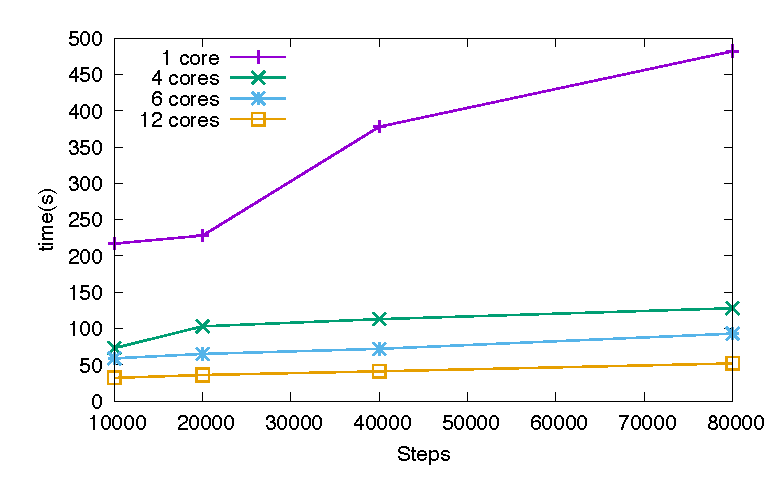
\includegraphics[width=1.0\linewidth]{Chap5/plots/scale.eps}}
\caption[Scalability of KNN2 code on Great Lakes HPC.]{Scalability of KNN2 code for 108,000 atoms on Great Lakes HPC from the University of Michigan with 2x 3.0 GHz Intel Xeon Gold 6154 processors and InfiniBand HDR100 networking, capable of 100 Gb/s throughput.}
\label{Chap:Al/Vac:fig:scale}
\end{figure}
\endgroup

